%! Author = bedlamzd
%! Date = 15.03.2021

\documentclass[14pt]{extarticle}
\usepackage{hyperref}

% Preamble
%! Author = bedlamzd
%! Date = 16.02.2021

\usepackage{fontspec}
\usepackage{polyglossia}
\defaultfontfeatures{Ligatures=TeX}
\setdefaultlanguage{russian}
\setotherlanguage{english}
\setmainfont{PT Astra Serif}
\newfontfamily{\latinfont}{PT Astra Serif}
\newfontfamily{\cyrillicfont}{PT Astra Serif}
\newfontfamily{\cyrillicfonttt}{FreeMono}

\usepackage{geometry}

\usepackage{mathtools}
\usepackage{amsmath}
\usepackage{amssymb}
\usepackage{amsfonts}
\usepackage{graphicx}
\usepackage{float}
\usepackage{wrapfig}
\usepackage{subcaption}

\geometry{right=20mm}
\geometry{left=20mm}
\geometry{top=20mm}
\geometry{bottom=20mm}

\usepackage{indentfirst}
\usepackage[outputdir=out]{minted}

\usepackage{booktabs}
\usepackage{array}

\renewcommand{\theFancyVerbLine}{\ttfamily{\normalsize\oldstylenums{\arabic{FancyVerbLine}}}}
\renewcommand{\listingscaption}{Листинг}

\newminted{python}{autogobble, linenos, fontsize=\small}
\newmintinline{python}{fontsize=\small}
\newmintedfile{python}{autogobble, linenos, fontsize=\small, breakanywhere, breaklines}

\newminted{lua}{autogobble, linenos, fontsize=\small}
\newmintinline{lua}{fontsize=\small}
\newmintedfile{lua}{autogobble, linenos, fontsize=\small, breakanywhere, breaklines}

%\renewcommand{\thesubsection}{\arabic{subsection}}

\graphicspath{{../img/}}



% Document
\begin{document}

    \begin{titlepage}
    \begin{center}
        \begin{small}
            \textbf{Министерство науки и высшего образования Российской Федерации}

            \vspace{1em}

            ФЕДЕРАЛЬНОЕ ГОСУДАРСТВЕННОЕ АВТОНОМНОЕ ОБРАЗОВАТЕЛЬНОЕ\\
            УЧРЕЖДЕНИЕ ВЫСШЕГО ОБРАЗОВАНИЯ

            \vspace{1em}

            \textbf{<<НАЦИОНАЛЬНЫЙ ИССЛЕДОВАТЕЛЬСКИЙ УНИВЕРСИТЕТ ИТМО>>}
        \end{small}

        \vspace{13ex}

        Лабораторная работа №1\\
        по дисциплине <<Имитационное моделирование робототехнических систем>>
    \end{center}

    \vspace{14em}

    \begin{flushright}
        \noindent
        Выполнил:\\
        студент гр. R41341c\\
        Борисов М. В.

        \vspace{1em}
        Преподаватель:\\
        Бжихатлов И. А.
    \end{flushright}

    \vfill

    \begin{center}
        \large{Санкт-Петербург}\\
        2021 г.\\
    \end{center}
\end{titlepage}


    \section*{Цель работы}
    \begin{itemize}
        \item Импортировать модель манипулятора в симулятор
        \item Собрать визуальную и физическую части манипулятора
        \item Написать скрипт для поиска зелёного куба в рабочем пространстве
        \item Реализовать касание манипулятором до куба при обнаружении
    \end{itemize}

    \section*{Ход работы}

    Воспользуемся моделью манипулятора доступной по ссылке
    \href{https://grabcad.com/library/robotic-arm-manipulator-fanuc-m-20ib-industrial-robot-1}{https://grabcad.com/library/robotic-arm-manipulator-fanuc-m-20ib-industrial-robot-1}
    и изображённом на рисунке~\ref{pic:man render}.

    \begin{figure}[H]
        \centering
        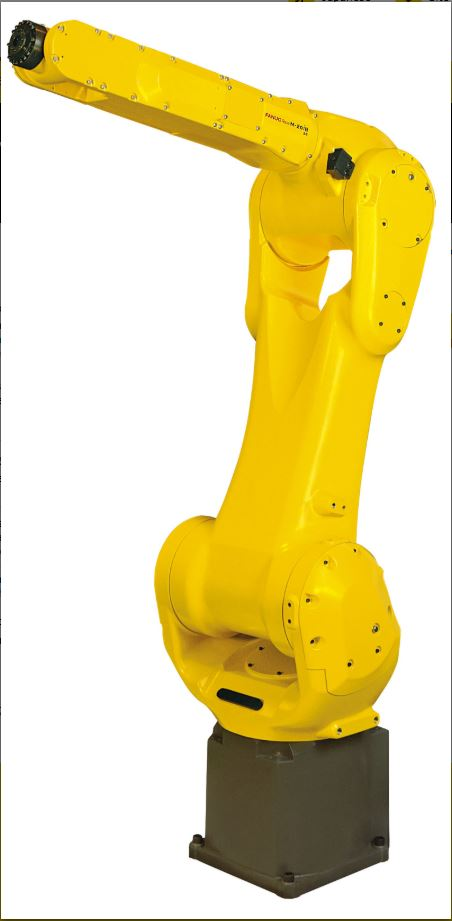
\includegraphics[height=0.4\textwidth]{man render.JPG}
        \caption{Рендер манипулятора}
        \label{pic:man render}
    \end{figure}

    Для уменьшения потребления ресурсов на рендер уменьшим число полигонов модели с помощью опции \texttt{Edit $\rightarrow$ Decimate selected shape}.
    Покрасим отдельные детали в различные цвета для удобства, после чего сделаем ещё более простые модели деталей. Эти
    детали будут служить физической репрезентацией манипулятора и на их основе будут считаться коллизии и взаимодействия.

    Базу робота заменим обычным цилиндром, остальные детали заменим их выпуклой оболочкой. Используя редактор вершин и
    мешей разметим места для установки осей вращения с помощью компонента \texttt{Dummy}. По ним в дальнейшем будет
    проще ориентироваться.

    Также с помощью этого компонента отметим конец последнего звена манипулятора, куда обычно крепятся инструменты. В
    это место мы прикрепим датчики.

    Все детали манипулятора необходимо называть шаблонно (рисунок~\ref{pic:tree}), в коде это упростит работу.

    В конечном итоге получим модель манипулятора и соответствующее ей дерево (рисунок~\ref{pic:man result}).

    \begin{figure}[H]
        \centering
        \begin{subfigure}{0.5\linewidth}
            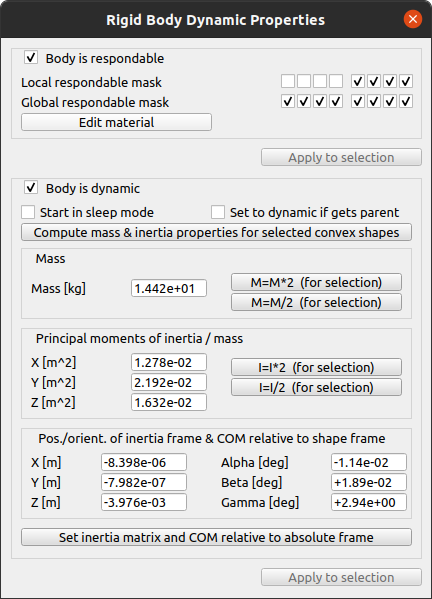
\includegraphics[height=0.35\textheight]{dyn setts.png}
            \caption{Настройки динамических компонентов}
            \label{pic:dyn setts}
        \end{subfigure}%
        \begin{subfigure}{0.5\linewidth}
            \centering
            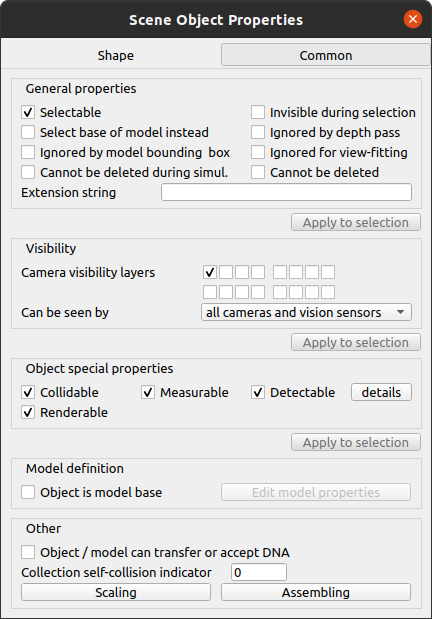
\includegraphics[height=0.35\textheight]{object setts.png}
            \caption{Настройки объекта измерения (куба)}
            \label{pic:cube setts}
        \end{subfigure}
        \begin{subfigure}{0.5\linewidth}
            \centering
            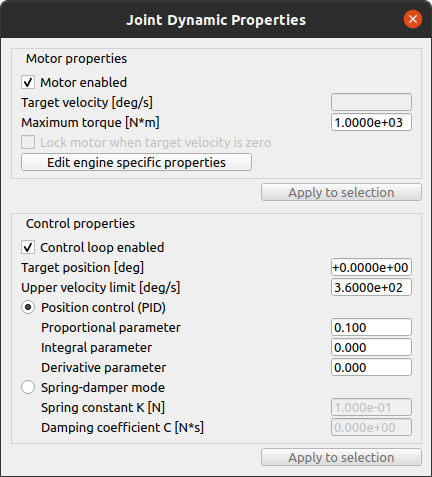
\includegraphics[height=0.35\textheight]{joint setts.png}
            \caption{Настройки сочленений}
            \label{pic:joint setts}
        \end{subfigure}
        \caption{Настройки тел и сочленений}
        \label{pic:settings}
    \end{figure}

    \begin{figure}
        \centering
        \begin{subfigure}{0.5\linewidth}
            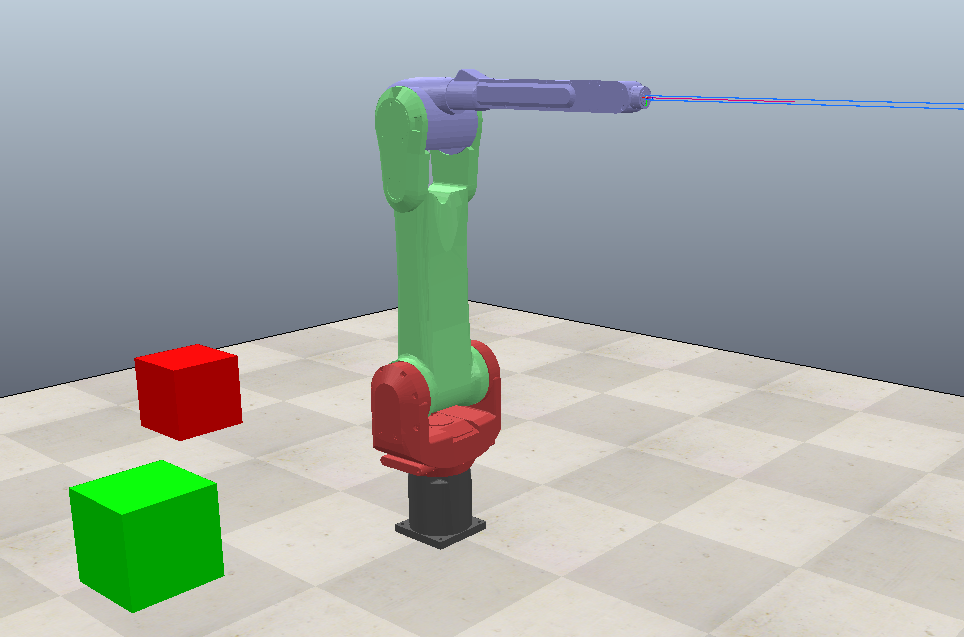
\includegraphics[height=0.35\textheight]{vrep model.png}
            \caption{Собранный манипулятор}
            \label{pic:vrep man}
        \end{subfigure}%
        \begin{subfigure}{0.5\linewidth}
            \centering
            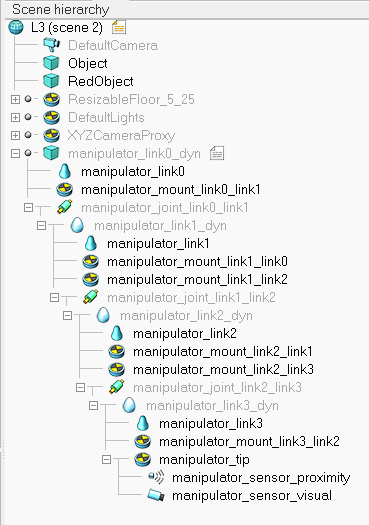
\includegraphics[height=0.35\textheight]{tree.png}
            \caption{Дерево модели манипулятора}
            \label{pic:tree}
        \end{subfigure}
        \caption{Модель}
        \label{pic:man result}
    \end{figure}

    На рисунке~\ref{pic:settings} показаны настройки для различных тел модели. При том для динамических тел, которые
    участвуют в расчётах важно чередование локальной маски соседних элементов для избежания ложных коллизий. Для
    элементов визуализации галочки динамики и взаимодействия сняты, поскольку в расчёте они не участвуют.

    Скрипт напишем с использованием remote API на python. Код целиком приведён в приложении~\ref{code:remoteAPI}.
    Алгоритм следующий:
    \begin{enumerate}
        \item Начать вращение вокруг своей оси (первое сочленение)
        \item Совершать осциллирующее движение последним звеном (сканировать пространство)
        \item Как только обнаружен зелёный куб остановиться
        \item Медленно приблизиться и коснуться куба
        \item Вернуться в исходное положение
    \end{enumerate}

    У данного алгоритма есть множество недостатков, в частности для "честного" касания куба необходимо решать обратную
    задачу кинематики. Также для "честного" определения зелёного предмета желательно переводить получаемый цвет в
    HSV пространство, которое даёт более надёжные измерения цвета. Однако в рамкой лабораторной работы такого алгоритма
    достаточно.

    Для каждого этапа алгоритма в скрипте прописана соответствующая функция, что позволяет при необходимости легко
    модифицировать и улучшить код (например, для последующих лабораторных работ).

    \section*{Вывод}
    В работе изучен алгоритм импорта сторонних файлов и создания из них моделей для симуляции. Изучена работа с новым
    визуальным сенсором. Разработан простой алгоритм взаимодействия с окружением и рассмотрены его недостатки.


    \appendix
    \renewcommand{\thesection}{\Asbuk{section}}


    \section{RemoteAPI скрипт}\label{code:remoteAPI}
    \pythonfile[frame=single]{../src/main.py}


\end{document}
